\documentclass[10pt]{developercv} % Default font size, values from 8-12pt are recommended

\begin{document}

\begin{minipage}[t]{0.8\textwidth}
  \vspace{-\baselineskip} % Required for vertically aligning minipages

  {\HUGE\textbf{\MakeUppercase{Ricardo Erikson}}}
  \vspace{5pt}

  {\huge Senior Software Engineer} % Career or current job title
\end{minipage}
\begin{minipage}[t]{0.2\textwidth}
  \vspace{-\baselineskip} % Required for vertically aligning minipages

  \begin{tikzpicture}[baseline=(pic.center),inner sep=0pt]
    \clip (0,0)  circle (1.5cm) node (pic) {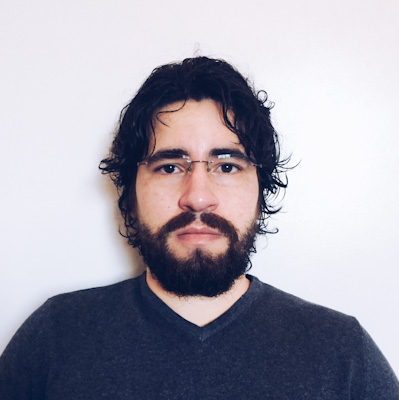
\includegraphics[width=3cm]{pic.jpg}};
  \end{tikzpicture}
\end{minipage}

\begin{minipage}[t]{0.4\textwidth}
  \vspace{-2.5\baselineskip} % Required for vertically aligning minipages

  \icon{MapMarker}{8}{Teresina, PI, Brazil}\\
  \icon{Phone}{8}{+55 92 98226 1492}\\
  \icon{At}{8}{\href{mailto:ricardo@ricardoerikson.me}{ricardo@ricardoerikson.me}}\\
\end{minipage}
\begin{minipage}[t]{0.4\textwidth}
  \vspace{-2.5\baselineskip} % Required for vertically aligning minipages

  \icon{Globe}{8}{\href{https://ricardoerikson.me}{ricardoerikson.me}}\\
  \icon{Github}{8}{\href{https://github.com/ricardoerikson}{github.com/ricardoerikson}}\\
  \icon{Linkedin}{8}{\href{https://linkedin.com/in/ricardoerikson}{linkedin.com/in/ricardoerikson}}\\
\end{minipage}

% \vspace{0.5cm}

\cvsect{Who Am I?}

\begin{minipage}[t]{\textwidth}
  % \vspace{-\baselineskip} % Required for vertically aligning minipages

  I have 15 years of experience working as a software engineer. I've had the opportunity to collaborate with key players of the software industry by building software for the web, mobile devices, distributed systems, and cloud environments. I'm looking for positions to evolve my career and skills with the following stack: Golang, Python, JavaScript, TypeScript, Angular, React, AWS, and Docker.
\end{minipage}
% \hfill % Whitespace between

\cvsect{Top Technical Skills}

\begin{minipage}[t]{\textwidth}
  % \vspace{-\baselineskip} % Required for vertically aligning minipages

  \begin{skills}
    \skillset{Languages}{Golang, Python, JavaScript, TypeScript}
    \skillset{Cloud (AWS)}{Cognito, EC2, ECR, CodeArtifact, CodeBuild, CodeDeploy, CodePipeline, RDS}
    \skillset{Databases}{MSSQL, MySQL, MariaDB, Postgres}
    \skillset{Frontend}{React, Angular}
    \skillset{CSS}{Bootstrap, Tailwind}
    \skillset{Other}{Docker, Git}
  \end{skills}
\end{minipage}

%----------------------------------------------------------------------------------------
%	EXPERIENCE
%----------------------------------------------------------------------------------------

\cvsect{Experience}

\begin{entrylist}
  \entry
  {2/2021 -- present\\\footnotesize{Remote}\\\footnotesize{Part-time}}
  {Front-end Engineer | DevOps Engineer}
  {Furukawa Electric LatAm}
  {Working as a front-end engineer using Angular and building CI/CD pipelines. Key achievements:\\
    \begin{contributionlist}
      \contribution{Built the authentication workflow using AWS Cognito.}
      \contribution{Built the deployment pipeline using AWS cloud environment.}
    \end{contributionlist}\\
    \texttt{Angular}\slashsep\texttt{AWS}\slashsep\texttt{Linux}}
  \entry
  {11/2020 -- present\\\footnotesize{Remote}}
  {Tech Lead | Golang Engineer}
  {BairesDev Inc.}
  {Working with Abbott's US cloud solutions team (BairesDev's client). Key achievements:\\
    \begin{contributionlist}
      % \contribution{helped the team to develop and maintain the API and the asynchronous services (messaging platform) of a scalable and high-traffic distributed system.}
      \contribution{Reduced the overall system overload by splitting long-running operations into batches of smaller ones.}
      \contribution{Improved the API security by identifying and fixing brute force attack vulnerabilities.}
    \end{contributionlist}\\
    \texttt{Golang}\slashsep\texttt{Docker}\slashsep\texttt{EC2}\slashsep\texttt{Python}}
  \entry{8/2016 -- 10/2020}
  {Sabbatical | Ph.D. Research | Trading Career}
  {}
  {
    I took a professional sabbatical to improve my academic qualifications and apply my programming knowledge to other areas. Key achievements:\\
    \begin{contributionlist}
      \contribution{Developed a 4-year Ph.D. research in the area of recommender systems where I had the opportunity to use Python (Pandas, NumPy, SciPy, and scikit-learn) to perform extensive data analysis and data visualization to build recommendation models.}
      \contribution{Started a career in the financial market as a sole trader exploring algorithmic trading and building data analysis tools with Python.}
    \end{contributionlist}\\
    \texttt{Python}\slashsep\texttt{Flask}\slashsep\texttt{Pandas}\slashsep\texttt{NumPy}\slashsep\texttt{Docker}\slashsep\texttt{Angular}}
  \entry{6/2015 -- 7/2016\\\footnotesize{Manaus, AM, Brazil}}
  {Senior Software Engineer}
  {IATECAM}
  {
    Worked as a senior software engineer, full-stack web developer in web projects using Java, and PHP. Key achievements:\\
    \begin{contributionlist}
      \contribution{Participated in key projects that helped the company to achieve the Level G of the MPS.BR, a QA certification program created by SOFTEX.}
      \contribution{Helped to define source code comment styling and a branching model to track project features from requirements to source code using Git.}
    \end{contributionlist}\\
    \texttt{Java}\slashsep\texttt{PHP}\slashsep\texttt{JavaScript}\slashsep\texttt{Angular}}
  \entry
  {3/2008 -- 5/2015\\\footnotesize{Manaus, AM, Brazil}\\\footnotesize{Part-time}}
  {Research Assistant}
  {Digital Television Laboratory - UFAM}
  {
    Worked as a research assistant of the Special Interest Group on Software Engineering, Embedded Systems and Automation (SEESA) at the Digital Television Laboratory.
  }
  \entry{11/2013 -- 3/2015\\\footnotesize{Manaus, AM, Brazil}}
  {Lead Software Engineer}
  {CETELI -- Samsung R\&D Center}
  {
    Worked as a technical lead in software projects for mobile and web platforms. I was responsible for making technical decisions with Java, JavaScript, HTML, CSS, and PHP. Key achievements:\\
    \begin{contributionlist}
      \contribution{Built the configuration management process, and the infrastructure for the CI/CD pipelines in development and testing environments.}
    \end{contributionlist}\\
    \texttt{Java}\slashsep\texttt{PHP}\slashsep\texttt{JavaScript}\slashsep\texttt{Android}}
  \entry{4/2010 -- 8/2012\\\footnotesize{Manaus, AM, Brazil}}
  {Tech Lead}
  {CETELI -- Nokia Institute of Technology}
  {
    Worked as a tech lead in software projects for mobile devices. Key achievements:\\
    \begin{contributionlist}
      \contribution{Coordinated and developed 30 mobile apps for Nokia devices that were published in the Nokia Ovi Store.}
    \end{contributionlist}\\
    \texttt{Qt}\slashsep\texttt{QML}\slashsep\texttt{JavaScript}\slashsep\texttt{HTML}\slashsep\texttt{CSS}}
  \entry{8/2007 -- 2/2008\\\footnotesize{Teresina, PI, Brazil}}
  {Freelance Web Developer}
  {Mundi Tecnologia}
  {Worked as a web developer using technologies such as PHP, HTML, CSS, and JavaScript.\\
    \texttt{PHP}\slashsep\texttt{JavaScript}\slashsep\texttt{HTML}\slashsep\texttt{CSS}}
\end{entrylist}

%----------------------------------------------------------------------------------------
%	EDUCATION
%----------------------------------------------------------------------------------------

\cvsect{Education}

\begin{entrylist}
  \entry
  {02/2021\\\footnotesize{Belo Horizonte, \\MG, Brazil}}
  {Ph.D Degree\\Electrical Engineering}
  {Federal University of Minas Gerais}
  {Research area: Recommender Systems}
  \entry
  {08/2010\\\footnotesize{Manaus, AM, Brazil}}
  {Master's Degree\\Electrical Engineering}
  {Federal University of Amazonas}
  {Research area: Software Components and Design Patterns}
  \entry
  {12/2006\\\footnotesize{Teresina, PI, Brazil}}
  {Technologist Degree\\Systems Analysis and Development}
  {Federal Institute of Technology of Piauí}
  {Research area: Digital Television}
\end{entrylist}

%----------------------------------------------------------------------------------------
%	ADDITIONAL INFORMATION
%----------------------------------------------------------------------------------------

\begin{minipage}[t]{0.3\textwidth}
  \vspace{-\baselineskip} % Required for vertically aligning minipages

  \cvsect{Languages}

  \begin{skills}
    \skillset{Portuguese}{native}
    \skillset{English}{fluent}
    \skillset{German}{elementary}
  \end{skills}
\end{minipage}

\end{document}
